\section{Introduction}
\label{s:intro}


% \wajih{I see some inconsistent Notations in this section. Please make sure that in this section all notations are up to date.}


% \wajih{Is there a difference between Semantic Harmonization or \wordvec Harmonization? You use \wordvec harmonization here and Semantic Harmonization in Design section. Let's use consistent terminology throughout the paper. }

% \wajih{There is a word "categorized ensemble learning" in the evaluation paragraph that is never described before in the intro. Let's use consistent wording througout the intro and throughout the paper. Also, in the Design section if you need to change the headings/titles to match with the intro, please do that. It is really hard to match the Intro section with the Design section.}

% \wajih{Terminology discrepancies are shown in green color throughout the paper.}

% \wajih{"Semantic Harmonization" vs. "Word2vec Harmonization"}

% \wajih{"Categorized Ensemble Learning" vs. "Categorization-based GNN Ensemble"}

% \wajih{"encoder" vs. "model"}

% \wajih{"GNNglobal" vs. "GNNGlobal":}

% \wajih{Categorized Provenance Subgraph" vs. "Process Entity Categorization"}

% \wajih{"FL using Categorized Process Entities" vs. "Categorized GNN-based Federated Learning"}

% \wajih{"Featurization" vs. "Semantic Encoding"}

% \wajih{"Central Server" vs. "Main Server"}

% \wajih{"Utility Server" vs. "Trusted Utility Server"}

% \wajih{"Semantic Attribute Vectors" vs. "Feature Vectors"}

% \wajih{"Dual-server Architecture" vs. "Two-server Architecture"}




%\wajih{I have updated the macro logs as it does not make sense to use \ logs for just "system". I have changed the macro to "system logs". Make sure the paper is consistent with that.}

% The effectiveness of IDSes hinges on their ability to accurately detect these threats, maintain low false positive rates, and operate with minimal resource consumption, ensuring system performance is not compromised.

%\wajih{Give the workflow of MSSP and cite that organizations outsource their security. If you find any numbers on how many comapnies use MSSP and outsource their security operations that would be great. If you find any realworld attack examples on MSSP where the data was leaked that would be great as well. }

\wajih{Highlight in the intro that as contribution that we provide formal privacy analysis our system. }


Intrusion Detection Systems (\ids) are crucial for countering Advanced Persistent Threats (APTs) in enterprises, as highlighted by major attacks~\cite{solarwinds,notpetya}. To strengthen defenses, many organizations turn to Managed Security Service Providers (MSSPs). A survey~\cite{msspsurvey} of over 5,000 IT professionals found that 75\% of companies use MSSPs. These providers integrate with client systems and typically configure them to transmit \logs to the cloud for centralized analysis. Figure~\ref{mssp} illustrates this MSSP architecture.



Recently, Provenance-based IDS (\pids)~\cite{streamspot,provdetector2020,wang2022threatrace,shadewatcher,yangprographer,han2020unicorn,jia2023magic,flash2024,cheng2023kairos,sigl} have proven highly effective by leveraging the rich contextual information in \logs. These systems transform \logs into provenance graphs and apply machine learning, particularly Graph Neural Networks (\gnnshort), to learn benign behavior patterns. By continuously monitoring these patterns, \pids can detect deviations that may indicate potential security threats. Upon detecting such anomalous graph patterns, the \pids generates alerts to prompt further investigation.

\smallskip
\PP{Critical Limitations of Existing \pids}
\smallskip

\noindent
Despite \pids potential, the current operational mode of MSSPs and the state-of-the-art \pids face significant challenges in enterprise settings, which are described below.

\noskipheading{1. Privacy Risks \& Centralization.} Current \pids depend on centralized infrastructure, requiring clients to transmit logs to a central server for aggregating large datasets and enabling deep learning models to capture benign behavior. This design introduces serious privacy risks, as logs often contain sensitive information, such as URLs, IP addresses, and application usage. These concerns are supported by a recent Datadog report~\cite{datadog}. Moreover, training on single-machine data is insufficient. Our experiments with \flash~\cite{flash2024} on the DARPA \optc dataset~\cite{darpaoptc} show a 40\% F-score drop when using single-host data compared to multi-host data.

\noskipheading{2. Network Overheads.}
Many \pids face critical challenges with network overhead and bandwidth constraints. Transmitting large volumes of logs for intrusion detection imposes high costs on users and organizations. Modern systems can produce gigabytes of logs daily~\cite{inam2023sok,hossain+depend}. Our analysis of \flash~\cite{flash2024} and \kairos~\cite{cheng2023kairos} using the \optc dataset (Section~\ref{cost_metric}) highlights these issues. Organizations similar in scale to those in the \optc dataset generate up to 1000 GB of logs daily, leading to significant network expenses. Users with limited bandwidth face difficulties uploading such large amounts efficiently.

\noskipheading{3. Scalability Issues.}
As the number of hosts increases, centralized \pids suffer from log congestion, resulting in detection delays and high storage demands. \flash and \kairos took 27.7 and 56.6 hours, respectively, to process a single day's OpTC logs. These extended processing times compromise effective threat detection and response capabilities, particularly in large-scale environments.



\smallskip
\PP{Combine FL with PIDS: Opportunity and Challenges}
\smallskip

\noindent
A seemingly promising solution to mitigate privacy and scalability limitations in centralized \pids is to integrate Federated Learning (FL) into their design. In such a federated \pids framework, each client constructs its local provenance graph, encodes semantic attributes using local feature sets \( \mathcal{F}_i \), and trains a local Graph Neural Network model \( \text{GNN}_{i} \). These clients then transmit only their model updates, rather than raw logs, to a central server, where the updates are aggregated into a global model \( \text{GNN}_{\text{global}} \). This approach preserves data locality and reduce bandwidth while enabling collaborative learning across multiple hosts. However, simply combining FL and \pids introduces several new challenges that hinder effectiveness:

\begin{figure}[t!]
  \centering
  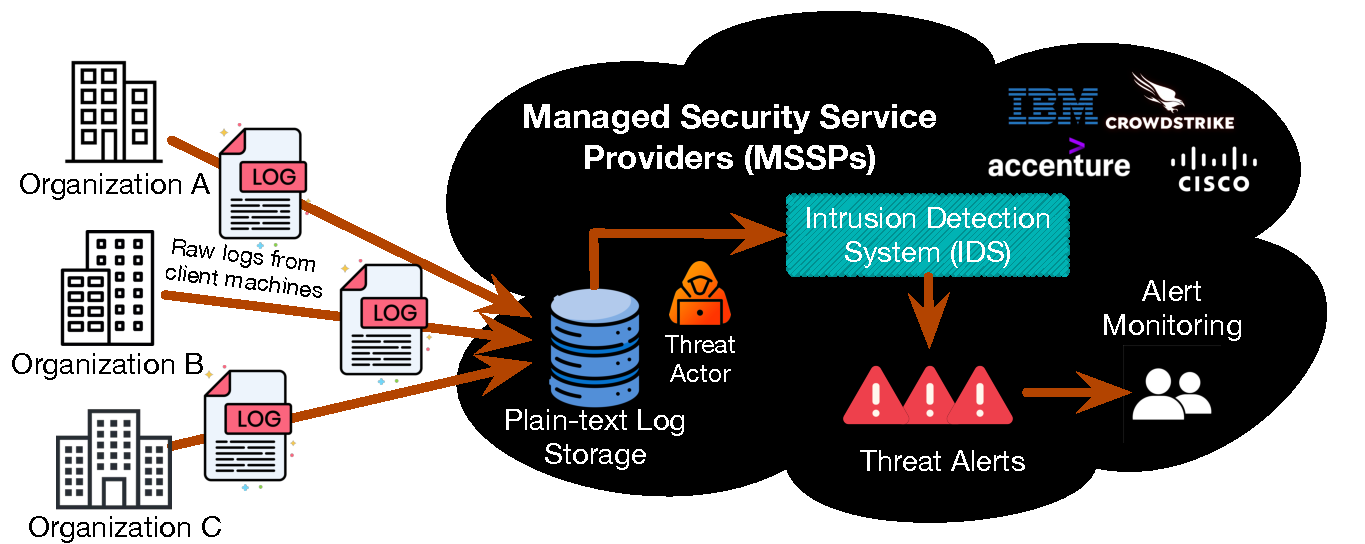
\includegraphics[width=0.42\textwidth]{fig/mssp.pdf}
  \caption{The MSSP architecture for intrusion detection collects plain-text system logs in a centralized storage managed by the MSSP. These system logs are then analyzed for intrusions. The architecture risks privacy leaks if a threat actor or a curious analyst within the MSSP accesses the logs.}
  \label{mssp}
  \vspace{-4ex}
\end{figure}


\begin{enumerate}[itemsep=0.1em, parsep=0em, topsep=0em, leftmargin=*]
  \labitem{C1}{itm:c1}{\it Data Imbalance \& Heterogeneity Among Clients.} Variations in data distribution and volume across clients, often non-IID~\cite{zhao2018federated}, pose challenges in training a global model \( \text{GNN}_{\text{global}} \) that performs uniformly well. Heterogeneous data resulting from different client applications can lead to suboptimal performance~\cite{qu2022rethinking}, and data imbalances can cause models to be biased towards clients with more extensive datasets, potentially overlooking unique patterns in less-represented clients~\cite{duan2020self}. This issue is critical for \pids, as a biased \( \text{GNN}_{\text{global}} \) may result in high false alarms, undermining detection accuracy.

  \labitem{C2}{itm:c2}{\it Feature Space Heterogeneity.} Inconsistent encoding of identical features across clients leads to difficulties in model convergence and reduces the effectiveness of federated averaging. \pids, such as \flash~\cite{cheng2023kairos}, utilize a \wordvec model to encode semantic attributes within a provenance graph. Due to the inherent randomness of the \wordvec algorithm, identical tokens \( t \) are encoded into different vectors \( v_i(t) \) by each client \( i \), using their local feature sets \( \mathcal{F}_i \). This variability disrupts the convergence and efficacy of local \gnn models \( \text{GNN}_{i} \) and complicates federated averaging for the global \gnn model \( \text{GNN}_{\text{global}} \), leading to suboptimal anomaly detection performance, as detailed in \cite{zhou2023fedfa}.

  \labitem{C3}{itm:c3} {\it Temporal Misalignment.} Aggregating temporal graph models from clients with temporally misaligned data challenges the creation of a cohesive global model. Systems like \kairos \cite{cheng2023kairos} employ temporal graph neural networks (TGN) to trace the evolution of system provenance graphs. However, federated learning's application across fragmented and misaligned client data impedes effective federated averaging, leading to improper alignment when aggregating models trained on diverse temporal datasets. This results in a loss of temporal information and hinders the formation of a cohesive global model \( \text{GNN}_{\text{global}} \).
  
\end{enumerate}


\smallskip
\PP{Our Approach and Contributions}
\smallskip

\noindent
We present \Sys, a privacy-preserving \pids that address the core challenges of applying FL to \pids. Prior work~\cite{wang2022threatrace} shows that graph-based models outperform traditional ML methods~\cite{chowdhary2020natural, goodfellow2020generative} applied directly to system logs~\cite{deeplog2017, xia2019loggan}. Building on this insight, \Sys leverages Federated Provenance Graph Learning, combining FL’s decentralized architecture with powerful graph representation learning to capture the intricate relationships among system entities. All major computations, including training, take place locally on client machines, leveraging their resources for real-time threat detection. This decentralized approach allows \Sys to scale effectively as more hosts are added, with each utilizing its own computing power and storage.  {\it To the best of our knowledge, \Sys is the first system to achieve accurate, scalable, and privacy-preserving federated \pids.}

To address ~\ref{itm:c1}, we have designed a novel categorization-based \gnnshort ensemble learning framework (Section~\ref{sys:fpgl}). In this framework, each submodel is trained to specialize in learning system activities associated with specific process entities, which are standardized across all clients. This standardization is facilitated by a sophisticated process entity categorization scheme enabled by our dual-server architecture. Through this system, process entities from all clients are organized into  \( K_{cat} \) privacy-preserving bins. Each client then aligns its process nodes with these bins, constructs a provenance subgraph for each bin, and trains a \gnnshort model on these graphs. The models from all clients are then aggregated into  \( K_{cat} \) model pairs, forming a comprehensive global ensemble model set \( \text{GNN}_{\text{global}} \). This strategic approach ensures that models with similar data distributions are merged effectively, thereby maintaining the integrity of unique activity patterns across diverse client environments.\footnote{We compared our methods with existing solutions including FedProx~\cite{li2020federated} and FedOpt~\cite{asad2020fedopt} for addressing heterogeneity in FL settings and found that our techniques outperform these existing solutions, as detailed in Section~\ref{sec:fedalternatives}.}

%\wajih{In the following paragraph, make sure that you use consistent terminology that you used in the design section like harmonization, featurization, categorization. This paragraph one of the important paragraphs. make sure you highlight all the features of your systems in this paragraph.}


To tackle ~\ref{itm:c2}, we implement a \wordvec harmonization scheme utilizing a dual-server architecture (Section~\ref{sub:model:harmonization}). In this setup, a central server issues encryption keys to clients, allowing them to securely encode \wordvec tokens. Subsequently, a utility server processes these encrypted tokens to achieve a unified, privacy-preserving vector representation. This method ensures that sensitive data remains protected while facilitating accurate and consistent \wordvec encoding across different clients. To avoid the problem of \ref{itm:c3} arising from the use of temporal graph networks, \Sys employs an inductive graph neural network model~\cite{hamilton2017inductive}, which has been shown by prior work~\cite{flash2024,shadewatcher,wang2022threatrace} to offer good performance and is not affected by temporal dependencies. 

\smallskip
\PP{Evaluation Results}
\smallskip

\noindent
We evaluated \Sys using open-source datasets from \darpa, including E3~\cite{error3}, E5~\cite{bug5}, and \optc~\cite{anjum2021analyzing}. The evaluation covers four dimensions: (1) Accuracy, (2) Efficiency and scalability, (3) Robustness, and (4) Privacy. For accuracy, we compare \Sys against a vanilla privacy-preserving \pids baseline that combines FL with a state-of-the-art (SOTA) \pids. We find that \Sys significantly outperforms this baseline. Since existing SOTA \pids already achieve near-perfect detection accuracy, {\bf the primary goal of \Sys is to demonstrate that a privacy-preserving \pids can be built while maintaining similar performance.} Our results show that \Sys achieves an average precision of 96\% and recall of 97\%, matching the accuracy of centralized SOTA \pids. To evaluate efficiency and scalability, we show that \Sys achieves a 170-fold reduction in network communication costs compared to centralized systems. Its decentralized design enables much faster inference, bounded only by the slowest client. \Sys completes the full \optc dataset in a few minutes, while existing \pids require several hours. To evaluate robustness, we present a comprehensive analysis of \Sys’s resilience against adversarial attacks in Section~\ref{sec:adversarial}. We also examine how differential privacy affects detection accuracy. In Section~\ref{sec:privacy}, we provide a detailed analysis of the privacy guarantees offered by \Sys. In Appendix, we conduct an ablation study to assess the effectiveness of individual components such as \wordvec harmonization. We also demonstrate that our approach outperforms existing techniques for handling data heterogeneity in FL settings.

\PP{Availability} \url{https://anonymous.4open.science/r/TrustWatch/}
% The main contributions of our work are as follows:

% \begin{itemize}[topsep=.1ex,itemsep=-.1ex,leftmargin=*]
%     \item[--] To the best of our knowledge, we are the first to introduce federated provenance graph learning in the domain of IDS with our system, \Sys.
%     \item[--] We have introduced a novel \textbf{ensemble learning} and \textbf{process entity categorization} framework for dealing with diverse heterogeneous client data distributions.
%     \item[--] We developed a sophisticated \textbf{\wordvec harmonization framework} using a multi-server architecture for secure private aggregation of semantic attributes.
%     \item[--] We conduct a comprehensive evaluation of our technique on real-world datasets, demonstrating \Sys's effectiveness in detecting system threats while being scalable and privacy-preserving.
% \end{itemize}

%\url{https://anonymous.4open.science/r/TrustWatch}

% \begin{table}[t!]
%   \centering
%   \scriptsize
%     %\caption{Limitations of existing \pids. \wajih{Add in caption that which \pids are not specified in the table and why.}}
%     \caption{Existing \pids limitations. \flash and \kairos outperform other existing \pids systems ~\cite{wang2022threatrace,han2020unicorn,streamspot,yangprographer,shadewatcher,provdetector2020}. Also, they all suffer from data privacy leakage issues. Therefore, we have excluded these \pids from the table. }
%     \setlength{\tabcolsep}{10pt}
%       \begin{tabular}{ | c | c | c | c |}

%         \hline
%              & \bf Data & \bf Network  & \bf Scalability \\
%              & \bf  Privacy & \bf  Overhead &  \\
%         \hline
%         \hline
%         \disdet~\cite{dong2023distdet} & NO                       & LOW      & HIGH       \\
%         \hline
%         \flash~\cite{flash2024}     & NO            & HIGH             & MEDIUM      \\
%         \hline
%         \kairos~\cite{cheng2023kairos}     & NO            & HIGH             & LOW         \\
%         \hline
%         {\bf\Sys}  & YES                & LOW               & HIGH        \\
%         \hline
%       \end{tabular}
%       \label{tab:limitations}
%   \end{table}
